\documentclass[11pt]{article}
\usepackage[a4paper,margin=1in]{geometry}
\usepackage{hyperref}
\usepackage{longtable}
\usepackage{array}
\usepackage{listings}
\usepackage{xcolor}
\usepackage{graphicx}

\hypersetup{
  colorlinks=true,
  linkcolor=blue,
  urlcolor=blue,
  citecolor=blue
}

\lstset{
  basicstyle=\ttfamily\small,
  breaklines=true,
  columns=fullflexible
}

\title{AI-Powered Animated Video Generation System\\Agentic AI Semester Project 2026}
\author{Group 6\\i221326 Abdul Momin\\i220961 Hamza Naveed\\i221042 Maaz Ali\\i221053 Huzaifa Nasir}
\date{May 5, 2026}

\begin{document}
\maketitle
\tableofcontents
\newpage

\begin{abstract}
This report presents an end-to-end, agentic pipeline that converts a single natural-language prompt into a short animated film. The system is implemented as a five-phase workflow: story and script generation, audio synthesis and mixing, video composition, a full-stack web interface for orchestration, and an edit agent with undo and version history. Each phase reads and updates a shared JSON state, enabling re-runs and targeted edits without reprocessing the entire pipeline. The implementation integrates LLM-based planning, TTS, image generation, FFmpeg-based compositing, and a LangGraph-driven edit agent with tool execution and state snapshots.
\end{abstract}

\section{Introduction}
Creating animated video content traditionally requires multiple specialists and long production timelines. This project demonstrates how a multi-agent workflow can automate that pipeline for short animated films. Our system accepts a single prompt and outputs a composited MP4 while exposing phase-level control, progress updates, and edit functionality. The project is structured to be modular and testable, with a shared schema that connects all phases.

\section{System Overview}
The pipeline is implemented as five modules, each with clear responsibilities and inputs/outputs.

\begin{lstlisting}
User Prompt
   |
   v
Phase 1: Story + Script + Characters (LLM)
   |
   v
Phase 2: Dialogue TTS + BGM + Timing (Audio)
   |
   v
Phase 3: Scene Images + Animation + Sync (Video)
   |
   v
Phase 4: Web UI + Orchestration (FastAPI + React)
   |
   v
Phase 5: Edit Agent + Undo (LangGraph + State Manager)
\end{lstlisting}

Each phase can run independently using CLI scripts or through the web application, and every run updates a central JSON state object stored under \texttt{data/outputs/}.

\subsection{Architecture Diagram}
Figure~\ref{fig:architecture} summarizes the main components. The diagram image can be generated from the Mermaid source in Appendix~\ref{app:mermaid}.

\begin{figure}[h]
  \centering
  \IfFileExists{diagrams/architecture.png}{
    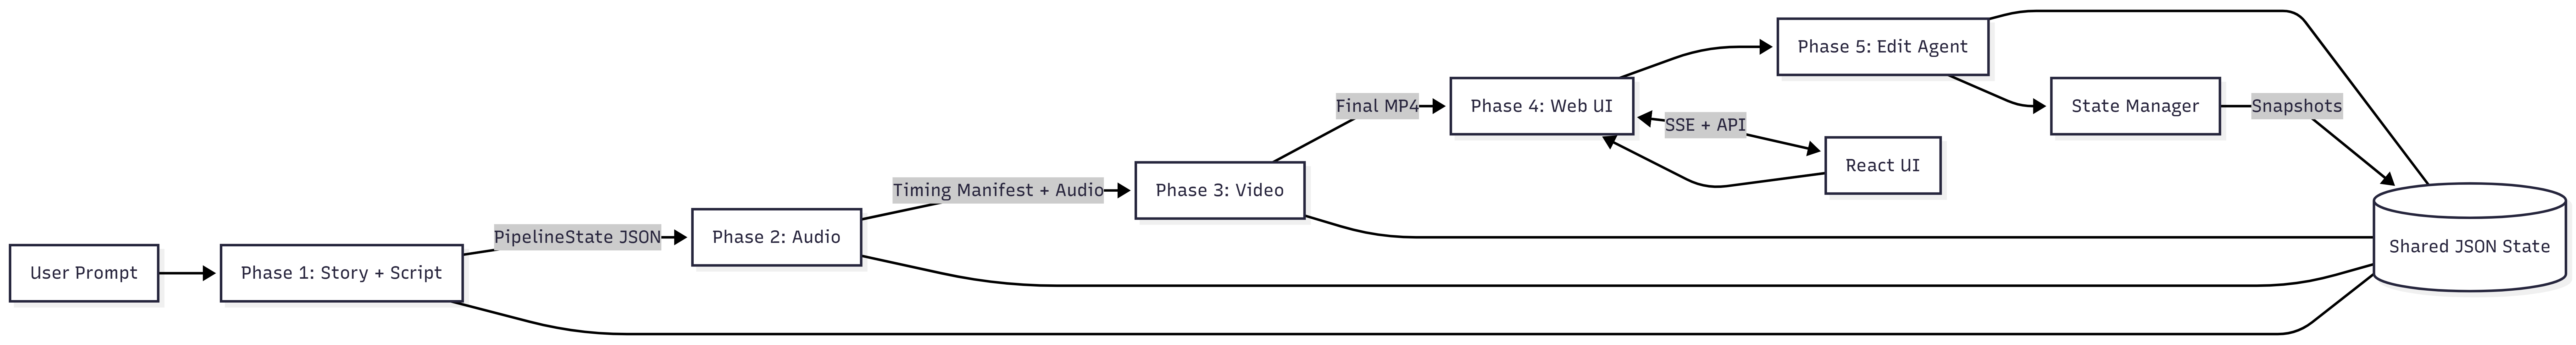
\includegraphics[width=0.95\linewidth]{diagrams/architecture.png}
  }{
    \fbox{\parbox{0.9\linewidth}{Architecture diagram placeholder. Export from Mermaid file: diagrams/architecture.mmd}}
  }
  \caption{End-to-end pipeline architecture and data flow.}
  \label{fig:architecture}
\end{figure}

\section{Shared JSON Schema}
A single JSON schema defines the contract between phases. It includes:
\begin{itemize}
  \item \textbf{meta}: project id, prompt, timestamps, schema version, duration, tags.
  \item \textbf{story}: logline, synopsis, genre, tone, and target duration.
  \item \textbf{characters}: id, name, role, voice profile, and visual profile.
  \item \textbf{scenes}: ordered scenes with setting, mood, visual prompt, and dialogue lines.
  \item \textbf{audio}: per-line audio references, BGM tracks, and a timing manifest.
  \item \textbf{video}: scene assets, final video path, subtitle information.
  \item \textbf{edits}: version history and current version id.
  \item \textbf{phases}: per-phase status and error metadata.
\end{itemize}

The schema is enforced via Pydantic models, with JSON Schema validation to ensure phase outputs are consistent. The schema enables selective re-runs and deterministic updates.

\subsection{Schema Excerpt}
The schema is implemented in \texttt{shared/schemas/pipeline\_state.schema.json}. Table~\ref{tab:schema} highlights the top-level fields and their roles.

\begin{longtable}{|p{0.22\linewidth}|p{0.70\linewidth}|}
\hline
\textbf{Field} & \textbf{Purpose} \\
\hline
meta & Project identifiers, timestamps, schema version, and total duration. \\
story & Logline, synopsis, tone, and target duration. \\
characters & Character roster with voice and visual profiles. \\
scenes & Ordered scenes with visual prompts and dialogue. \\
audio & Per-line audio assets, BGM tracks, and timing manifest. \\
video & Scene assets, subtitle data, and final MP4 path. \\
edits & Version history and snapshot metadata. \\
phases & Status map for phase progress and errors. \\
\hline
\caption{PipelineState top-level schema fields.}
\label{tab:schema}
\end{longtable}

\section{Phase 1: Story and Script Generation}
Phase 1 expands the user prompt into a structured narrative and scene plan. It uses a Groq-hosted LLM (model: \texttt{llama-3.3-70b-versatile}) with strict JSON formatting rules. The planner ensures:
\begin{itemize}
  \item 3--6 scenes totaling 15--45 seconds.
  \item 2--4 characters with consistent gender and visual descriptions.
  \item Scene dialogue lines linked to character ids.
  \item BGM moods normalized to a controlled vocabulary.
\end{itemize}

The output is validated and normalized before it becomes the canonical \texttt{PipelineState}. A repair pass is included to fix schema deviations from the LLM when necessary.

\section{Phase 2: Audio Generation and Integration}
Phase 2 converts dialogue into audio and assembles background music (BGM) for each scene. It performs:
\begin{itemize}
  \item TTS synthesis per dialogue line using ElevenLabs or an offline fallback.
  \item Timing manifest generation with start and end timestamps.
  \item Scene-level BGM selection by mood from a local library.
  \item Mixing of dialogue and BGM with configurable gain controls.
\end{itemize}

The phase writes per-line WAV files, per-scene mixes, and a final concatenated audio track. Outputs are stored under \texttt{data/outputs/phase2/<project\_id>/}.

\subsection{Audio Timing Strategy}
We compute a dialogue timeline by summing line durations and a configurable inter-line gap. The timing manifest aligns each dialogue line to a global timeline and becomes the source of truth for video synchronization. BGM is trimmed or padded to match scene duration so the final mixed audio remains consistent with scene timing.

\section{Phase 3: Video Generation and Composition}
Phase 3 renders scene visuals and synchronizes them with audio. The implementation includes:
\begin{itemize}
  \item Image generation with Pollinations, conditioned by scene prompts and character visuals.
  \item Per-speaker image prompts to align lip-sync and dialogue segments.
  \item Ken Burns style animation and concatenation using FFmpeg.
  \item Optional Wav2Lip integration for per-segment lip-sync.
  \item Subtitle generation and burn-in as an optional step.
\end{itemize}

Scene assets, clips, and final MP4 outputs are stored in \texttt{data/outputs/phase3/<project\_id>/} with metadata logs for prompt and lip-sync decisions.

\subsection{Visual Prompting Strategy}
We generate per-speaker prompts to ensure that each dialogue segment has a matching character image, which improves lip-sync quality and keeps character identity consistent. The prompts combine scene tone, camera framing, and character visual profiles.

\section{Phase 4: Web Interface and Orchestration}
The web interface provides a user-facing control plane for the pipeline. The backend is built with FastAPI and exposes:
\begin{itemize}
  \item Per-phase run endpoints and a full-pipeline endpoint.
  \item SSE streaming for live progress updates.
  \item State and video retrieval endpoints.
  \item Edit agent endpoints for classification and undo operations.
\end{itemize}

The frontend is built with React and Vite. It includes status cards, live event logs, a video preview panel, and edit and undo interfaces. The UI supports phase-level reruns and refreshes state and history from the backend.

\subsection{API Surface}
Table~\ref{tab:api} lists the core API routes implemented by the backend.

\begin{longtable}{|p{0.32\linewidth}|p{0.60\linewidth}|}
\hline
\textbf{Endpoint} & \textbf{Purpose} \\
\hline
GET /api/projects & List stored project ids, state paths, and video paths. \\
GET /api/status/\{project\_id\} & Phase status, errors, and latest artifacts. \\
GET /api/stream/\{project\_id\} & Server-sent events for live progress updates. \\
POST /api/run/phase1 & Run Phase 1 with a prompt. \\
POST /api/run/phase2 & Run Phase 2 for an existing project. \\
POST /api/run/phase3 & Run Phase 3 for an existing project. \\
POST /api/run/full & Execute all phases sequentially. \\
POST /api/edit & Submit a natural-language edit request. \\
POST /api/edit/undo & Revert to a previous snapshot version. \\
\hline
\caption{Core API endpoints.}
\label{tab:api}
\end{longtable}

\section{Phase 5: Edit Agent with Undo}
Phase 5 allows natural-language edits after the initial render. The edit agent uses LangGraph with tool bindings and a state manager for snapshots.

\subsection{Edit Flow Diagram}
Figure~\ref{fig:editflow} captures the classification and tool-execution loop. The diagram image can be generated from the Mermaid source in Appendix~\ref{app:mermaid}.

\begin{figure}[h]
  \centering
  \IfFileExists{diagrams/edit_flow.png}{
    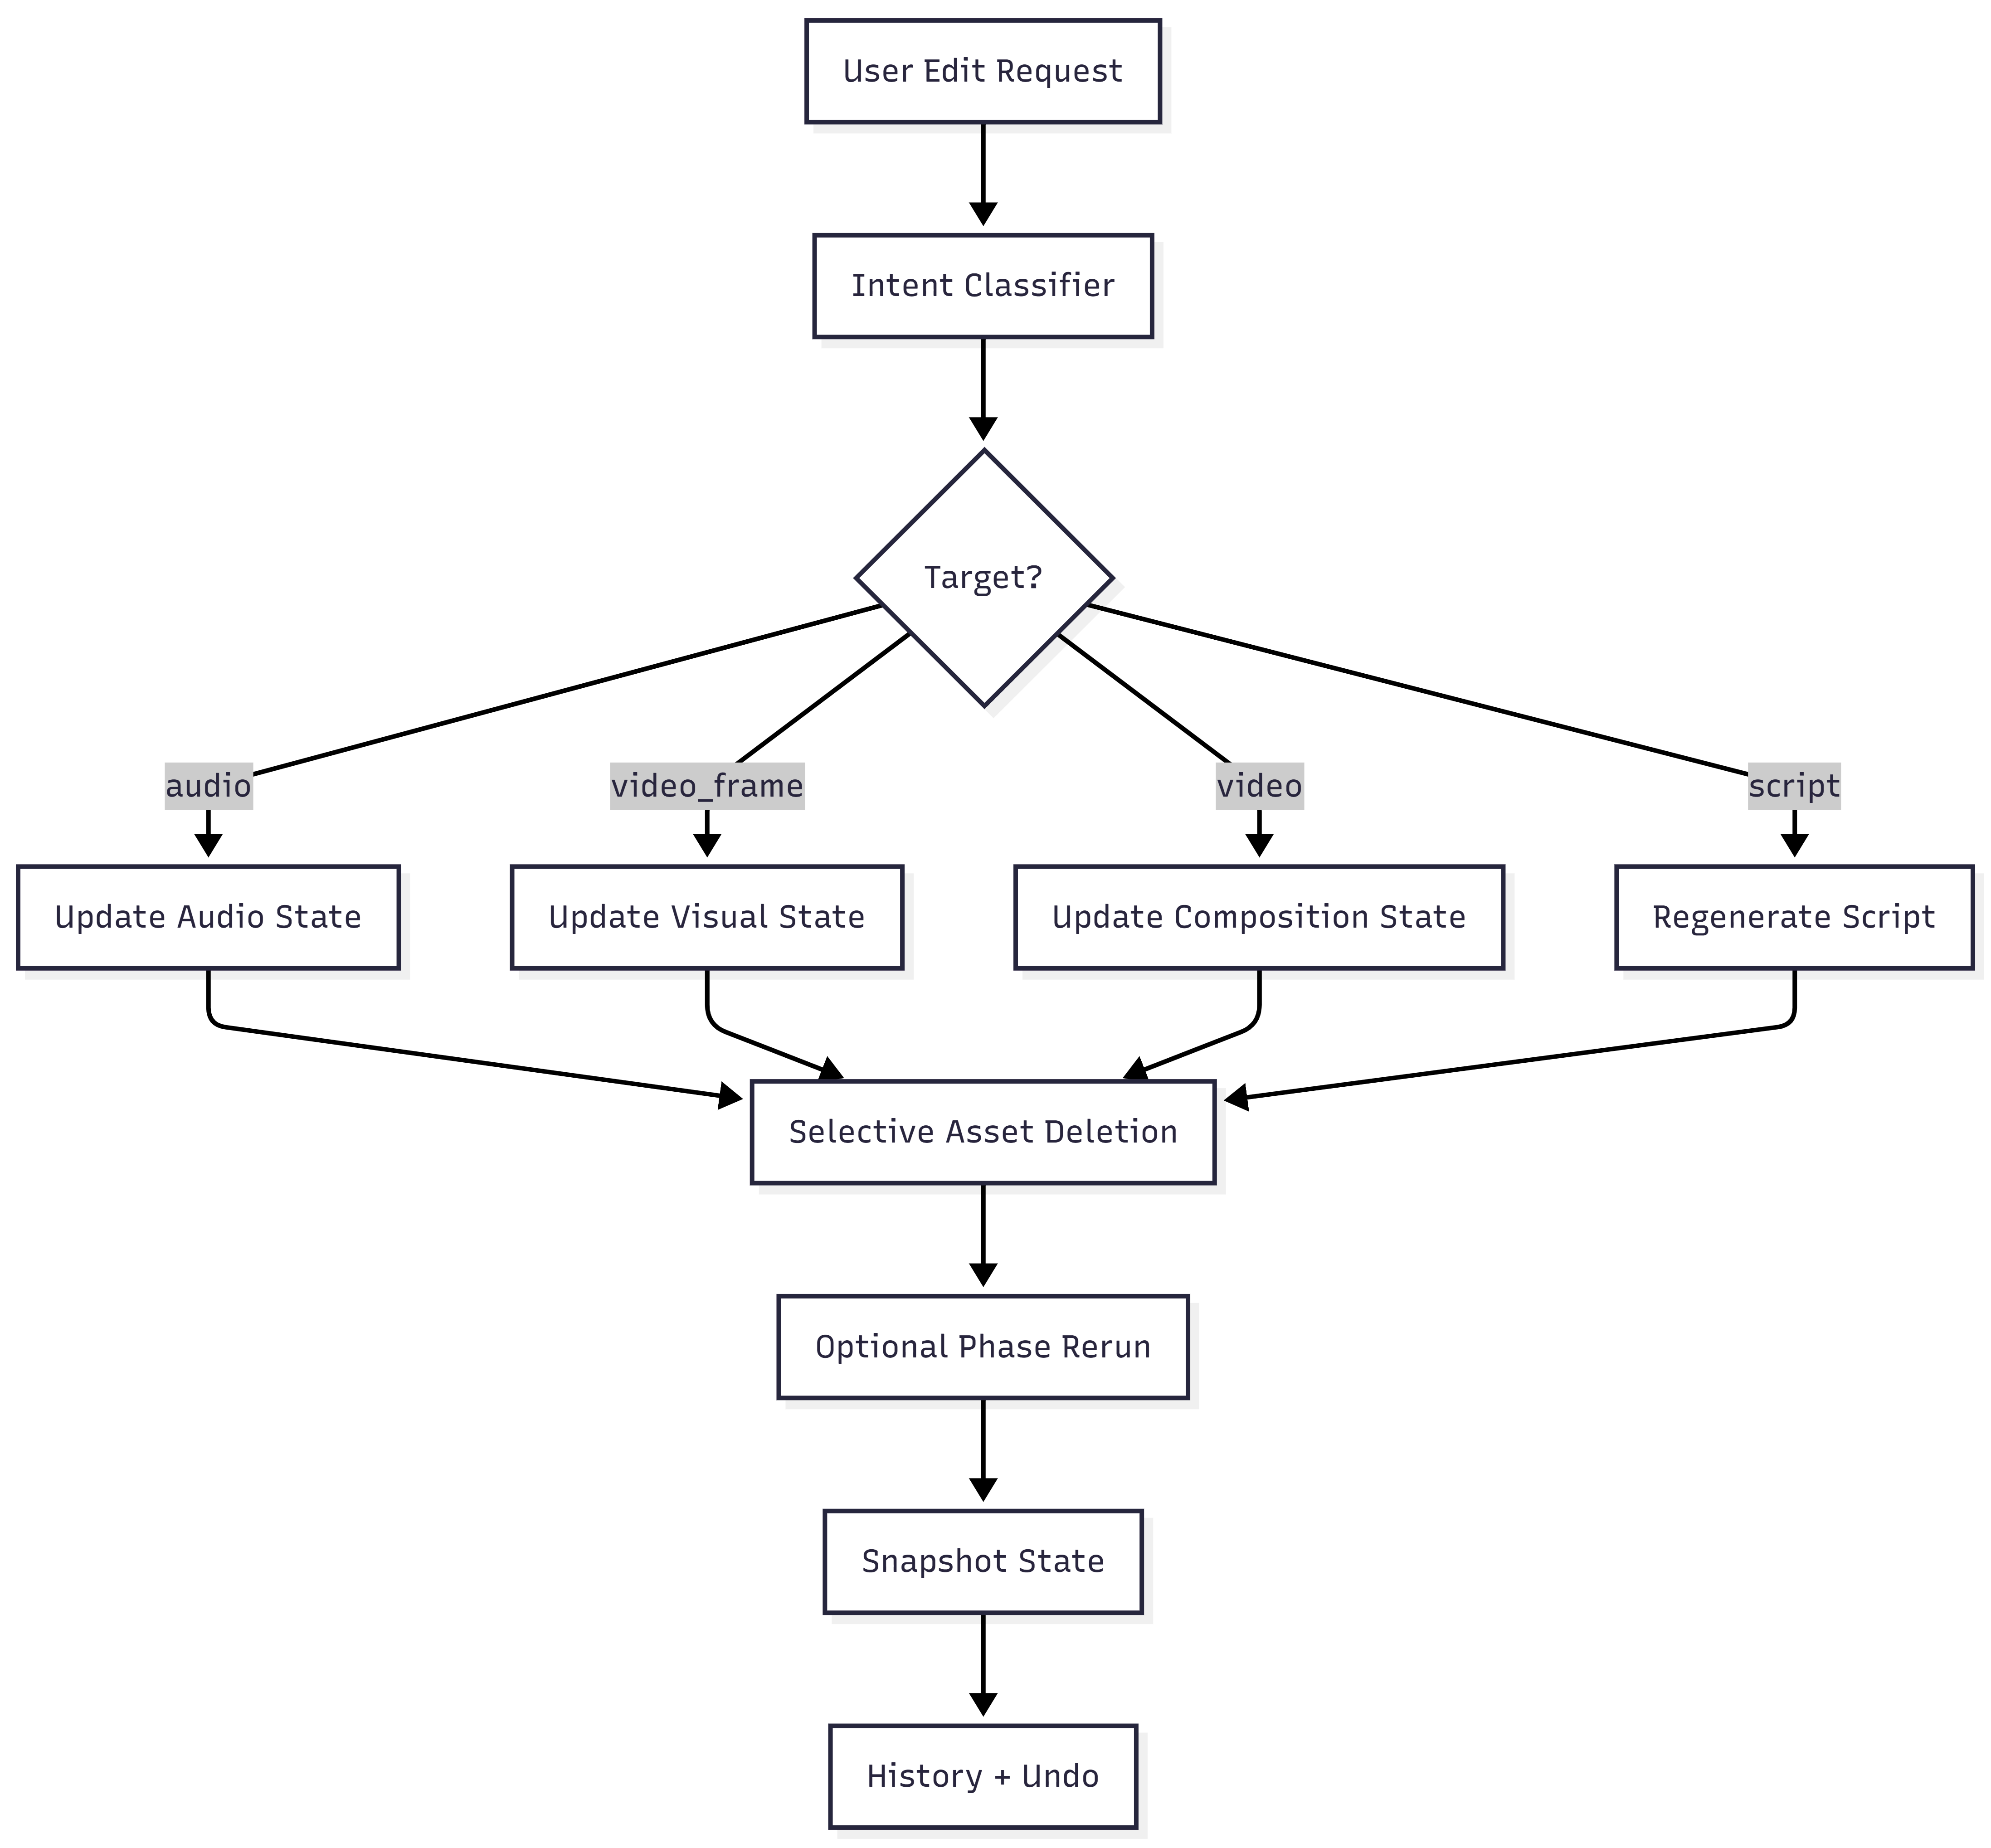
\includegraphics[width=0.95\linewidth]{diagrams/edit_flow.png}
  }{
    \fbox{\parbox{0.9\linewidth}{Edit agent flow diagram placeholder. Export from Mermaid file: diagrams/edit_flow.mmd}}
  }
  \caption{Edit agent classification and tool-execution loop.}
  \label{fig:editflow}
\end{figure}

\subsection{Intent Classification}
An LLM-based classifier parses edit requests into a structured object:
\begin{lstlisting}
{
  "intent": "change_voice_tone",
  "target": "audio",
  "scope": "character:char_1",
  "parameters": {"tone": "whispered"}
}
\end{lstlisting}

The classifier supports targets such as \texttt{audio}, \texttt{video\_frame}, \texttt{video}, and \texttt{script}. When ambiguity exists, the agent queries project context before taking action.

\subsection{Tool Execution and Selective Reruns}
The edit agent routes requests to tool functions that update the JSON state and delete targeted cached assets to force regeneration. Examples include:
\begin{itemize}
  \item Update scene background and delete affected images and clips.
  \item Update character visuals and remove dependent assets.
  \item Update voice tone and rerun audio generation.
  \item Update BGM mood and remux the video.
\end{itemize}

After state updates, the agent can re-run the appropriate pipeline phase on request.

\subsection{State Versioning and Undo}
The system maintains an append-only history of snapshots for each project. A snapshot captures the state JSON and all referenced assets. The UI exposes a history panel to revert to any prior version, restoring the exact pipeline state and files.

\subsection{Versioning Sequence}
Figure~\ref{fig:versioning} shows how snapshots are taken during edits and how a revert restores a previous state.

\begin{figure}[h]
  \centering
  \IfFileExists{diagrams/versioning.png}{
    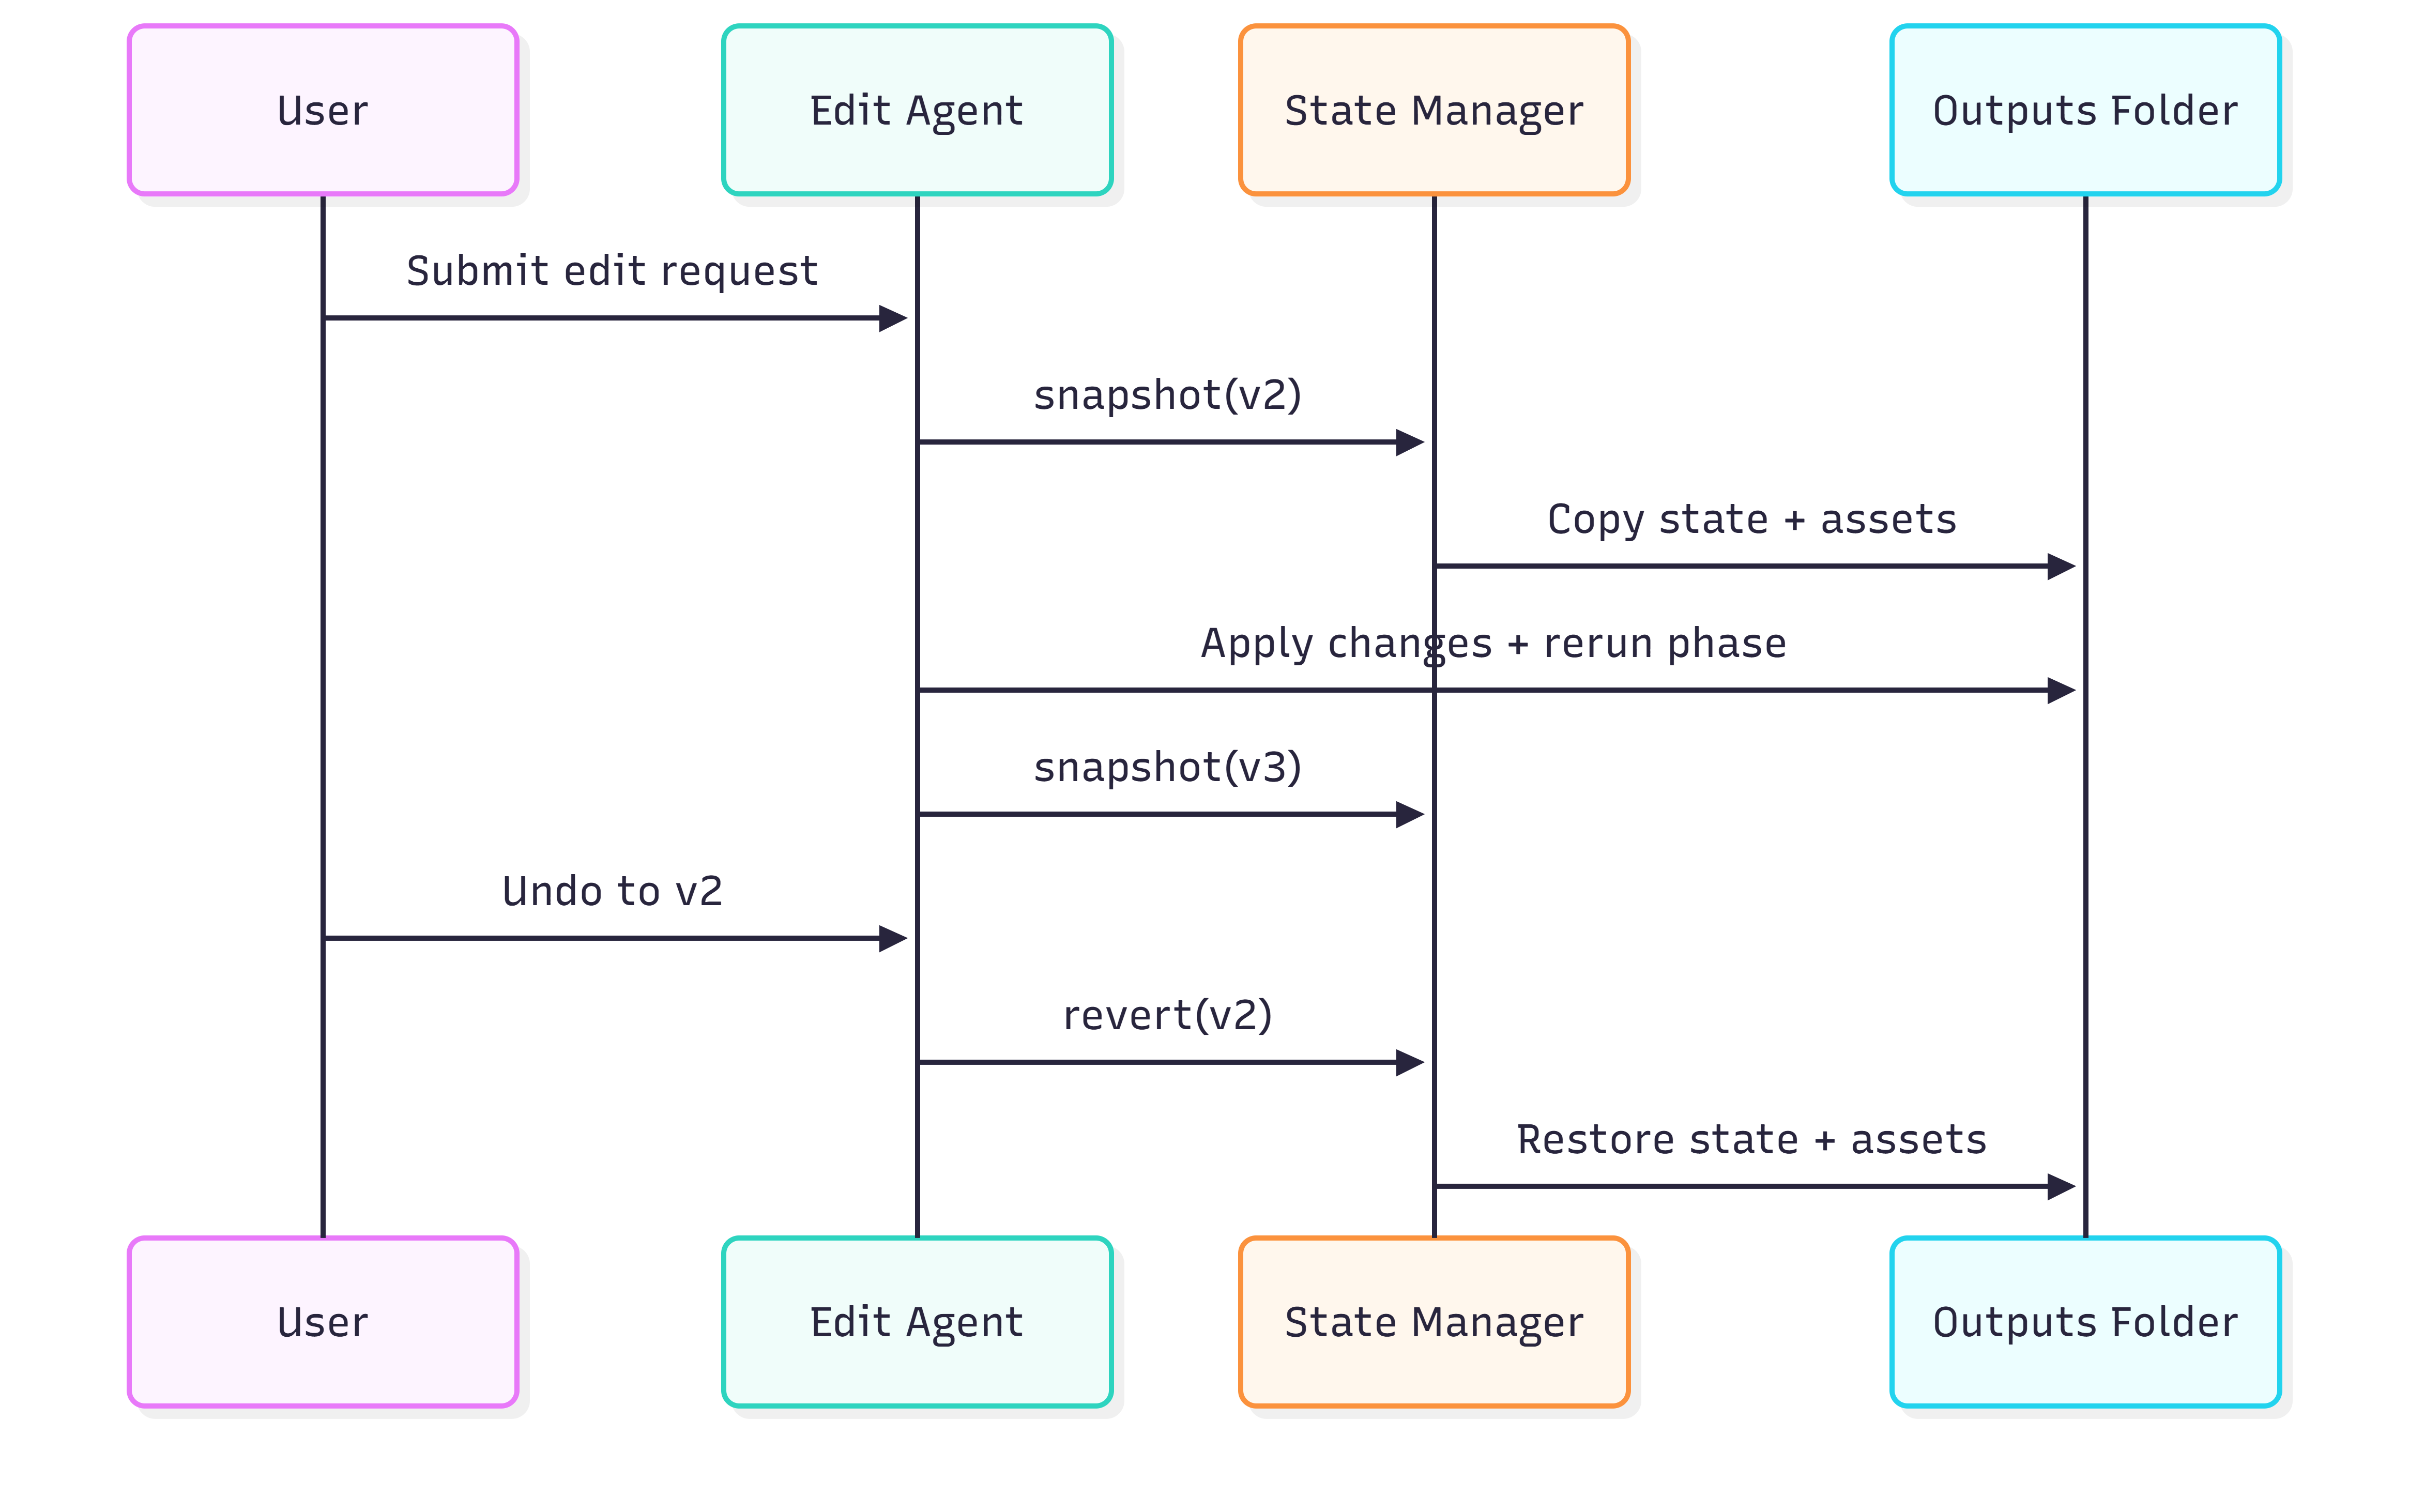
\includegraphics[width=0.95\linewidth]{diagrams/versioning.png}
  }{
    \fbox{\parbox{0.9\linewidth}{Versioning sequence diagram placeholder. Export from Mermaid file: diagrams/versioning.mmd}}
  }
  \caption{Snapshot and undo sequence.}
  \label{fig:versioning}
\end{figure}

\section{Orchestration and Execution}
Phase execution can be triggered via CLI scripts or via the web API. The backend maintains an in-memory job store and broadcasts progress over SSE. Each phase updates the state and writes a phase-complete record. The LangGraph edit graph runs with a SQLite checkpointer to preserve conversational context and tool call history.

\section{Testing}
Unit tests are provided for multiple agents, including story, audio, and video components, as well as edit intent classification. Tests verify schema validity, tool routing behavior, and pipeline state updates. Test files are located under \texttt{agents/*/tests} and \texttt{tests/}.

\subsection{Test Coverage Summary}
Key test areas include:
\begin{itemize}
  \item Story agent JSON schema validation and normalization.
  \item Audio agent timing manifest and asset generation.
  \item Video agent asset creation and output paths.
  \item Edit intent classification for multiple query types.
  \item State manager snapshot and revert behavior.
\end{itemize}

\section{Results}
We verified the pipeline using the sample project \texttt{proj\_601cadb0}. The system produced:
\begin{itemize}
  \item A structured Phase 1 state JSON with validated characters and scenes.
  \item Full audio output with timing manifest and scene mixes.
  \item A composited MP4 video with optional subtitle burn-in.
  \item Successful edit requests with state snapshots and undo operations.
\end{itemize}

The outputs are stored in \texttt{data/outputs/phase1/}, \texttt{data/outputs/phase2/}, and \texttt{data/outputs/phase3/}. Phase-level reruns were verified through both CLI and the web interface.

\subsection{Visual Artifacts}
Figure~\ref{fig:datapath} provides a data flow view and where artifacts are produced in the repository. The diagram can be generated from Appendix~\ref{app:mermaid}.

\begin{figure}[h]
  \centering
  \IfFileExists{diagrams/data_flow.png}{
    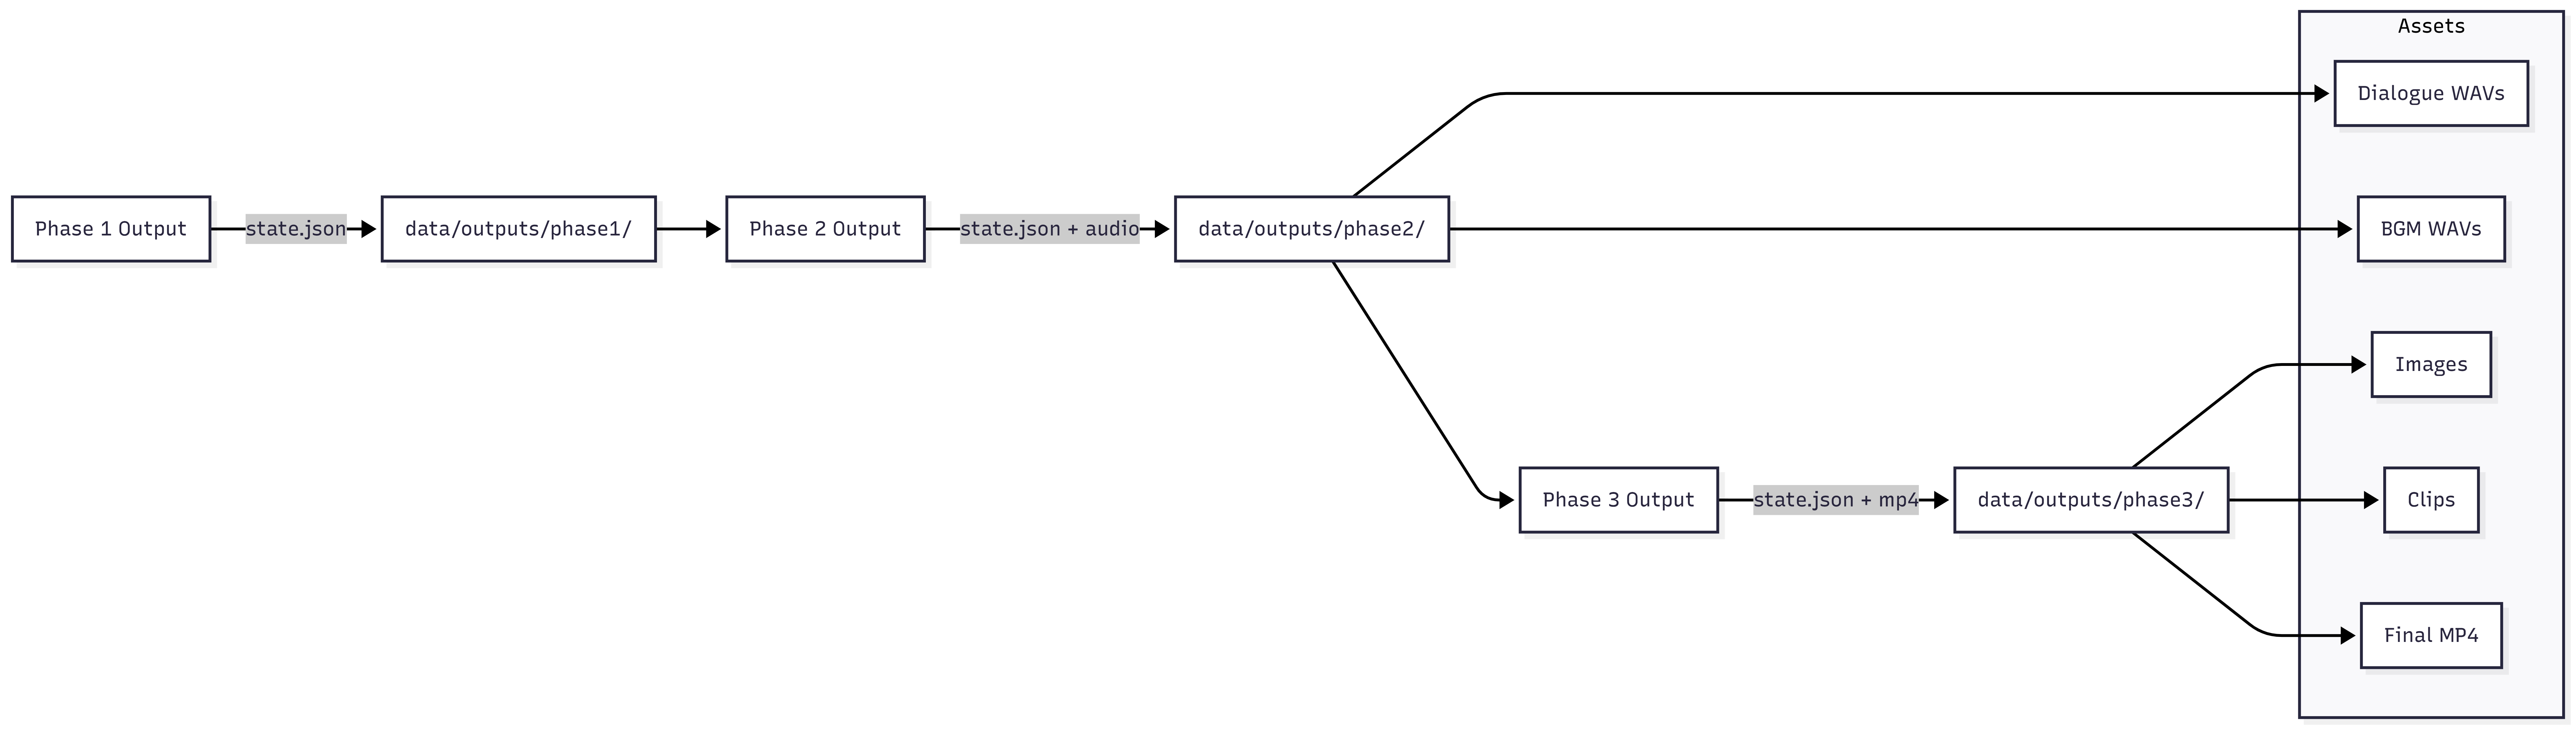
\includegraphics[width=0.95\linewidth]{diagrams/data_flow.png}
  }{
    \fbox{\parbox{0.9\linewidth}{Data flow diagram placeholder. Export from Mermaid file: diagrams/data_flow.mmd}}
  }
  \caption{Artifact flow across phases and outputs.}
  \label{fig:datapath}
\end{figure}

\section{Challenges and Mitigations}
\begin{itemize}
  \item \textbf{LLM output drift}: Implemented schema validation with repair prompts to enforce JSON structure.
  \item \textbf{Dialogue alignment}: Enforced speaker-turn segmentation to keep timing consistent.
  \item \textbf{Voice and visual consistency}: Normalized gender and aligned visual descriptors to voices.
  \item \textbf{BGM balance}: Exposed tunable gain controls and debug logging.
  \item \textbf{Edit safety}: Required context lookups and used targeted asset deletion to avoid full reruns.
\end{itemize}

\section{Limitations and Future Work}
\begin{itemize}
  \item Add richer visual variety per scene with multiple images and transitions.
  \item Improve lip-sync robustness and face detection fallbacks.
  \item Expand edit intents to include pacing, camera motion, and subtitle styling.
  \item Provide a Docker-based installer for easier deployment.
  \item Add richer evaluation metrics for story coherence and A/V sync quality.
\end{itemize}

\section{Individual Contributions}
All members collaborated across phases with shared ownership of the JSON schema and cross-phase integration. Each member contributed to design, implementation, testing, and documentation for their respective modules:
\begin{itemize}
  \item Abdul Momin
  \item Hamza Naveed
  \item Maaz Ali
  \item Huzaifa Nasir
\end{itemize}

\section{Conclusion}
This project demonstrates a complete, modular agentic pipeline for prompt-to-video generation. The shared state contract enables reliable handoff between phases, while the edit agent and undo system provide practical post-generation control. The system fulfills the requirements for a full-stack AI pipeline with multi-agent orchestration and serves as a foundation for further research and productization.

\section{Deliverables Checklist}
Table~\ref{tab:deliverables} maps the required artifacts to their locations in the repository or submission package.

\begin{longtable}{|p{0.35\linewidth}|p{0.55\linewidth}|}
\hline
\textbf{Artifact} & \textbf{Location / Notes} \\
\hline
GitHub repository & Public repo \texttt{AgenticAI\_Project\_Group\_6} (submit link). \\
Project report (PDF) & This report (exported from \texttt{Project\_Report.tex}). \\
Demo video (3--7 min) & Screen recording showing prompt-to-video, 3 edits, 2 undo. \\
Presentation slides & PDF or PPTX, 10--15 minutes demo flow. \\
Sample outputs & \texttt{data/outputs/phase1}, \texttt{phase2}, \texttt{phase3}. \\
Unit tests & \texttt{agents/*/tests} and \texttt{tests/}. \\
\hline
\caption{Submission artifacts required by the assignment.}
\label{tab:deliverables}
\end{longtable}

\appendix
\section{Mermaid Sources}
\label{app:mermaid}
This appendix includes the Mermaid source files used to generate figures. Render them locally or in a Mermaid-compatible tool and export PNGs to the \texttt{diagrams/} folder.

\subsection{Architecture Diagram}
\IfFileExists{diagrams/architecture.mmd}{
  \lstinputlisting{diagrams/architecture.mmd}
}{
  \noindent Mermaid source placeholder: diagrams/architecture.mmd
}

\subsection{Edit Agent Flow}
\IfFileExists{diagrams/edit_flow.mmd}{
  \lstinputlisting{diagrams/edit_flow.mmd}
}{
  \noindent Mermaid source placeholder: diagrams/edit\_flow.mmd
}

\subsection{Data Flow}
\IfFileExists{diagrams/data_flow.mmd}{
  \lstinputlisting{diagrams/data_flow.mmd}
}{
  \noindent Mermaid source placeholder: diagrams/data\_flow.mmd
}

\subsection{Versioning Sequence}
\IfFileExists{diagrams/versioning.mmd}{
  \lstinputlisting{diagrams/versioning.mmd}
}{
  \noindent Mermaid source placeholder: diagrams/versioning.mmd
}

\section*{References}
\begin{itemize}
  \item Groq API and LLM models
  \item ElevenLabs TTS
  \item Pollinations image generation
  \item FFmpeg and MoviePy tooling
  \item LangChain and LangGraph
  \item FastAPI and React
\end{itemize}

\end{document}
